\documentclass{cmspaper}
\usepackage{graphicx}
\usepackage{rotate}
\usepackage{relsize}
\usepackage{lineno}

\newcommand{\met} {\ensuremath{E\!\!\!\!/_T}}
\newcommand{\ttbar} {\ensuremath{t\bar{t}~}}
\newcommand{\ptll} {\ensuremath{P_T(\ell\ell)}}
\newcommand{\ptllres} {\ensuremath{P^{\rm res}_T(\ell\ell)}}
\def\ack{\section*{Acknowledgments}}

%\linenumbers


\begin{document}

%==============================================================================
% title page for many authors
%
\begin{titlepage}
\title{Inclusive search for Same-Sign Top Quark Pair Production using Dileptons at $\sqrt{s} = 7 $ TeV}

  \begin{Authlist}
    D.~ Barge, C.~Campagnari, P.~Kalavase, D.~Kovalskyi, V.~Krutelyov, J.~Ribnik
    \Instfoot{ucsb}{University of California, Santa Barbara}
    W.~Andrews, G.~Cerati, D.~Evans, F.~Golf, I.~MacNeill, S.~Padhi, Y.~Tu, F.~W\"urthwein, A.~Yagil, J.~Yoo
    \Instfoot{ucsd}{University of California, San Diego}
    L.~Bauerdick, I.~Bloch, K.~Burkett, I.~Fisk, Y.~Gao, O.~Gutsche, B.~Hooberman, S.~Jindariani
    \Instfoot{fnal}{Fermi National Accelerator Laboratory, Batavia, Illinois}
  \end{Authlist}

\begin{abstract}
Significant evidence of asymmetries in $t\bar{t}$ production have been recently 
reported by the Tevatron experiments.   They could be due to FCNC in the top
sector.  These new interactions
could imply an enhancement of  same-sign top pair production via 
the t-channel exchange of a non-universal 
massive neutral vector boson ($Z'$) at the LHC. 
This note presents the first inclusive search for same-sign top quark 
pair production using dileptons at the LHC. 
The study is performed using data corresponding to an integrated luminosity 
of 35 pb$^{-1}$ at $\sqrt{s} = 7 $ TeV recorded  by CMS in 2010. 
No excess above the standard model background expectation is observed. 
Limits are set on the propagator mass as a function of $Z'$ couplings to 
the standard model quarks at the 95\% confidence level. 
\end{abstract}
\end{titlepage}

\section{Introduction}
\label{sec:intro}

After the successful operation of the Large Hadron Collider (LHC) and the CMS detector
in 2010 and 2011, and with good prospects for the future, the LHC is now ready to shed light on a number 
of open questions in Particle Physics 
such as the mechanism of electroweak (EW) symmetry breaking, or the 
new physics, Beyond the Standard Model (BSM), that stabilizes the EW scale. 

A wealth of theories that extend the Standard Model have been put forth during the past decades. Supersymmetry (SUSY) is
arguably the best motivated BSM theory --- and certainly the most 
thoroughly studied. 
Indeed, searches for SUSY are among the primary objectives of the 
CMS experiment. SUSY is exceedingly popular not 
only for its theoretical beauty but also because SUSY phenomenology 
is extremely rich, 
%in fact is can mimic almost any other new physics scenario. 
leading to a large variety of possible new signals at the LHC. 
In spite of this, the majority of SUSY studies focus on a very special 
setup: the so-called Constrained Minimal Supersymmetric Standard Model (CMSSM). 
This was justified in the preparation for discoveries as the CMSSM, 
having just a handful of new parameters, is very predicive. However, 
the simplifying assumption of universality at the GUT scale lacks a sound 
theoretical motivation. Consequently, the CMSSM should be regarded as a showcase 
model. When it comes to interpreting experimental results, it is reasonable and interesting to do this within the CMSSM because it 
provides (to some degree) an easy way to show performances, 
compare limits or reaches, etc. However, the interpretation of experimental results in the 
$(m_0,m_{1/2})$ plane risks imposing unwarranted constraints on SUSY, as many 
mass patterns and signatures that are possible a priori are not covered in the CMSSM. 
The same problem arises in any analysis that assumes a particular 
SUSY breaking scheme. 

In this document, we therefore introduce a different approach, which uses only 
minimal assumptions on the underlying SUSY parameters. In particular, given the absence of experimental guidance, we choose
not to rely on a particular SUSY breaking scheme.
Instead, we use a 19-dimensional 
parametrization of the MSSM, called the \emph{phenomenological MSSM} (pMSSM),
with parameters defined not at the GUT scale but instead at the SUSY scale 
(by convention the geometric mean of the two stop masses).
We demonstrate the feasibility of our approach by applying it to 
the 2011 CMS data-set corresponding to 1~fb$^{-1}$ of integrated luminosity.  
Using profile likelihoods, we combine 
the dijet $\alpha_T$ analysis, the opposite-sign dilepton 
analysis and the same-sign dilepton analysis and derive constraints 
on the SUSY particles with as few simplifying assumptions as possible.
Results from other SUSY analyses in CMS will be added as soon as they become available.

We first give the motivation to go beyond the CMSSM and work in 
a generic MSSM setup. After this, the pMSSM and its parametrization is defined. 
We then outline our analysis, giving details on the pMSSM points we have used, 
the detector simulation and the CMS analyses, and describe the statistical method based on 
profile likelihoods used for coping with the 19-dimensional model. Finally, we discuss our results and summarize our conclusions.


\section{Monte Carlo event generation}
\label{sec:mc}

We used the external model interface in MadGraph~\cite{madgraph} 
to generate $pp \to tt$ and $pp \to ttj$ events at LO 
with the Lagrangian described in Equation \ref{eqn:L_berger} with $f_L = 0$, $f_R = 1$.  
Different values of $f_R$ were modelled by rescaling the cross-sections
for the t-channel (Fig.~\ref{fig:tchannel}) and s-channel (Fig.~\ref{fig:schannel}) 
by $f_R^4$ and $f_R^2$, respectively.
The range of $Z'$ masses considered was 100 GeV to 2 TeV in the t-channel
and 200 GeV to 2 TeV in the s-channel. 
The minimum mass cut is higher for the s-channel where
the $Z'$ boson decays to a top and a light flavour quark
to ensure the on-shell $Z'$ mass is always  larger than the top mass.

We used the CTEQ6L~\cite{cteq6l} parton distribution function (PDF)
and set the renormalization and factorization scales
to be at the top mass scale ($m_{t} = 172.5$ GeV). 
The width of the $Z'$ boson was calculated using 
BRIDGE~\cite{bridge} and verified the results with MadGraph~\cite{madgraph}. 
The generated events were fed to Pythia for 
parton showering.
The detector response was taken into account with the standard CMS
fast-simulation program.

The total production cross sections for $tt$ and $ttj$ 
at the leading-order (LO) are shown as a function of $Z'$ 
mass in Fig.~\ref{fig:sstopcross}. 
Our calculated cross sections agree well with the 
published literature~\cite{berger}. 

\begin{figure}[htb]
\begin{center}
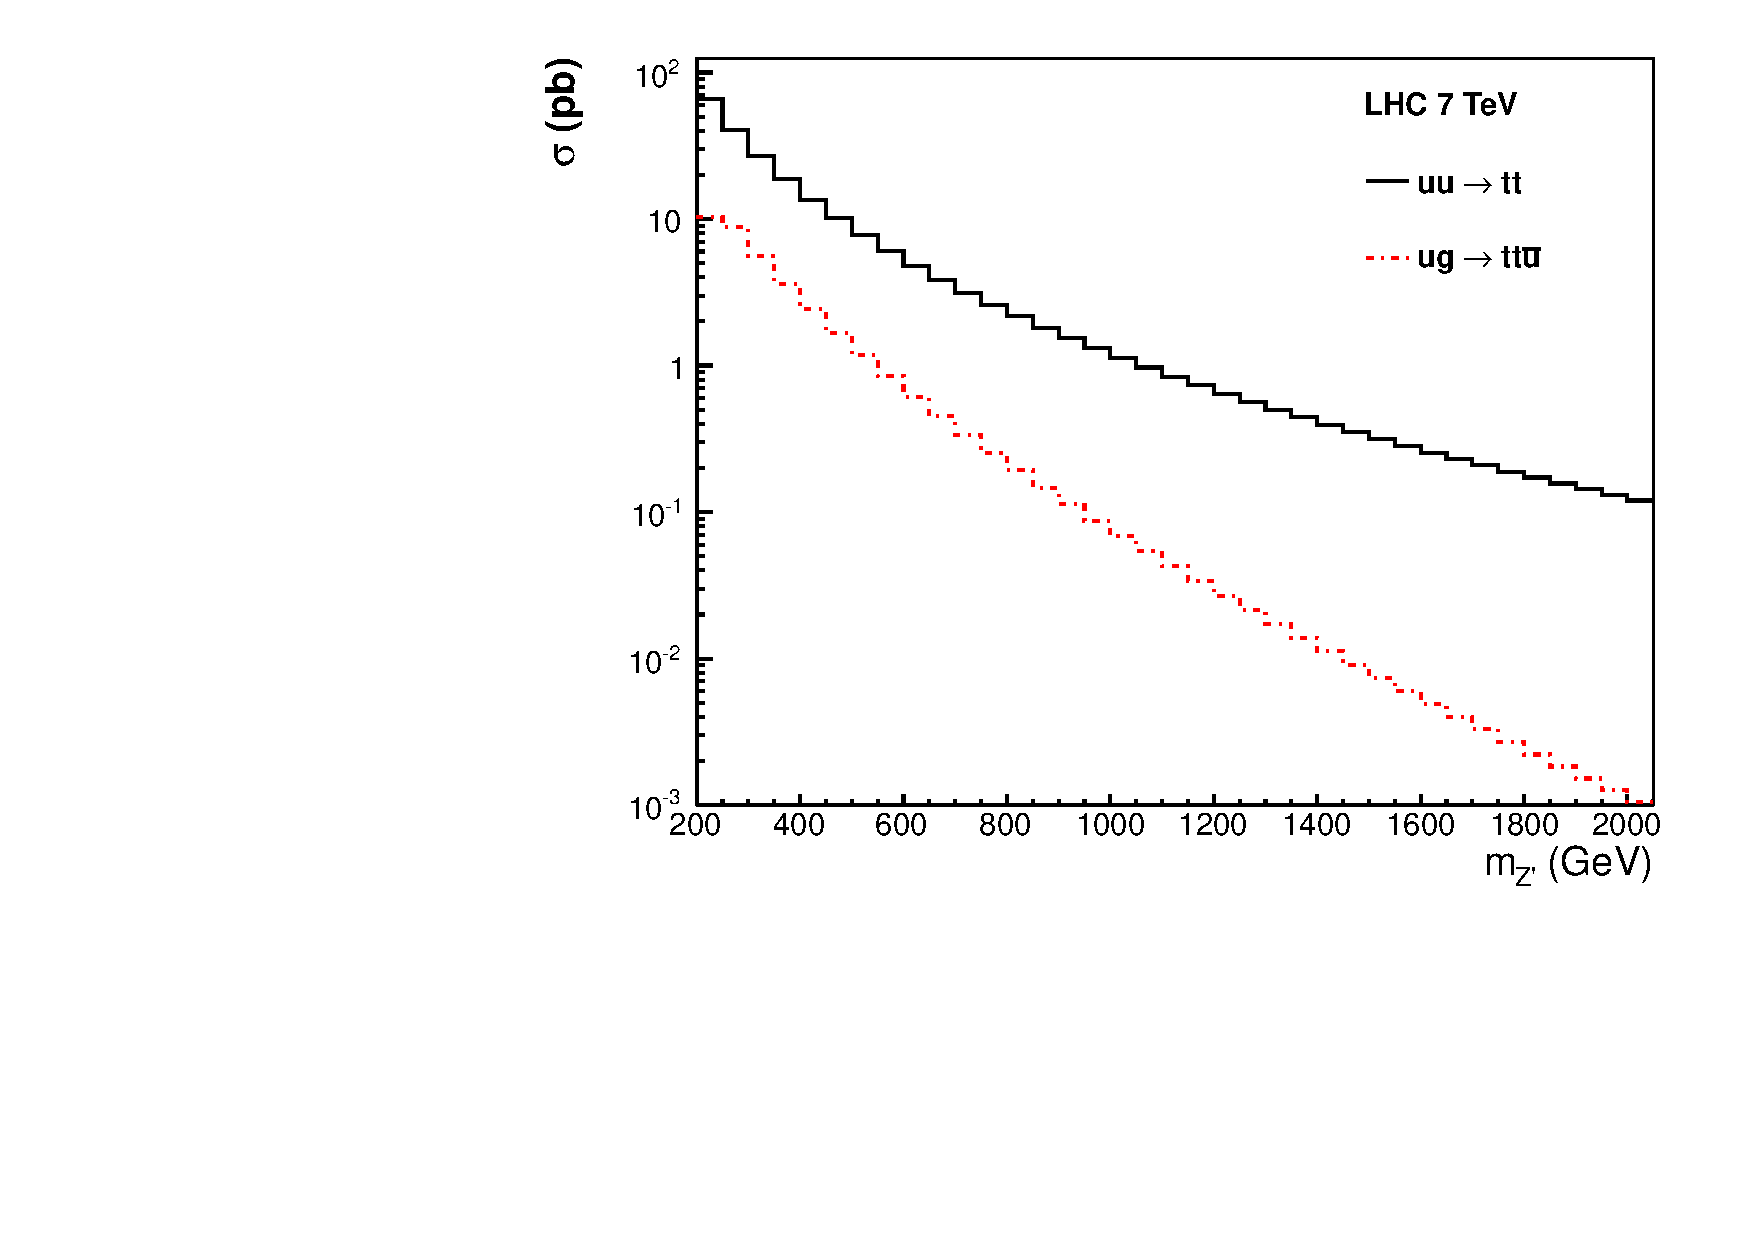
\includegraphics[width=0.7\linewidth]{figs/sstopcross.pdf}
\caption{ LHC production cross section for $tt$ and $ttj$ diagrams using right-handed coupling, $f_R = 1$. 
The renormalization and factorization scales are set to the top mass. \label{fig:sstopcross}}
\end{center}
\end{figure}
%%% commented out - DLE
%%%\section{Data Samples}
\label{sec:datasamples}
This study is based on the 2\_2\_X re-reco full simulation data samples
listed in Table~\ref{tab:datasets}.  The Standard Model (SM) data sets have been normalized 
to the cross-sections compiled by the top group~\cite{tosi};  for the SUSY 
data sets we used the cross-sections from the Summer 2008 production 
page~\cite{summer08}.

\begin{table}[hbt]
\begin{center}
\begin{tabular}{|l|}\hline
{\tt /TTJets-madgraph/Fall08\_IDEAL\_V11\_redigi\_v10/GEN-SIM-RECO} \\
{\tt /WJets-madgraph/Summer08\_IDEAL\_V11\_redigi\_v1/GEN-SIM-RECO} \\
{\tt /ZJets-madgraph/Summer08\_IDEAL\_V11\_redigi\_v1/GEN-SIM-RECO} \\
{\tt /WW/Summer08\_IDEAL\_V11\_redigi\_v1/GEN-SIM-RECO} \\
{\tt /WZ\_incl/Summer08\_IDEAL\_V11\_redigi\_v1/GEN-SIM-RECO} \\
{\tt /ZZ/Summer08\_IDEAL\_V11\_redigi\_v1/GEN-SIM-RECO} \\
{\tt /SingleTop\_sChannel/Summer08\_IDEAL\_V11\_redigi\_v3/GEN-SIM-RECO} \\
{\tt /SingleTop\_tWChannel/Summer08\_IDEAL\_V11\_redigi\_v3/GEN-SIM-RECO} \\
{\tt /SingleTop\_tChannel/Summer08\_IDEAL\_V11\_redigi\_v3/GEN-SIM-RECO} \\
{\tt /SUSY\_LM0-sftsht/Summer08\_IDEAL\_V11\_v1/GEN-SIM-RECO} \\
{\tt /SUSY\_LM*-sftsht/Summer08\_IDEAL\_V11\_redigi\_v1/GEN-SIM-RECO} \\
\hline
\end{tabular}
\caption{The data sets used in this study.\label{tab:datasets}}
\end{center}
\end{table}

Monte Carlo events were analyzed with CMSSW\_2\_2\_10 
with the additional tags listed in Table~\ref{tab:tags}.

\begin{table} [htb]
\begin{center} 
\begin{tabular}{|l|} \hline
{V01-08-04 CondFormats/JetMETObjects} \\
{V00-06-02-09 DataFormats/METReco} \\
{V07-02-12-03 DataFormats/MuonReco} \\
{V01-08-02-01 JetMETCorrections/Algorithms} \\
{V01-08-15 JetMETCorrections/Configuration} \\
{V03-02-06 JetMETCorrections/JetPlusTrack} \\
{V02-09-02 JetMETCorrections/Modules} \\
{VB04-00-02-04 JetMETCorrections/Type1MET} \\
{V01-04-03 RecoJets/JetAssociationAlgorithms} \\
{V00-04-02-17 RecoMET/Configuration} \\
{V02-05-00-21 RecoMET/METAlgorithms} \\
{V02-08-02-17 RecoMET/METProducers} \\
{V03-26-04 DataFormats/PatCandidate} \\
{V05-05-09 PhysicsTools/PatAlgos} \\
{V03-06-03 PhysicsTools/PatUtils} \\
{V03-01-16 PhysicsTools/PFCandProducer} \\
{V09-30-03 PhysicsTools/HepMCCandAlgos} \\
{V05-13-02 DataFormats/HepMCCandidate} \\
\hline
\end{tabular}
\caption{Additional software tags used in this study.\label{tab:tags}}
\end{center}
\end{table}

%%% commented out - DLE
%%%\section{Event Selection}
\label{sec:eventselection}

The event selection used is not optimized for any specific non-standard model 
scenario. It is based on small modifications to the baseline 
di-lepton event selection that we used in our same-sign published study~\cite{ssnote1, sspaper}. The 
only difference is that we now require both leptons to have the transverse 
momentum ($p_t$) $> 20$ GeV. A quick summary of the event selection is:

\begin{itemize}
\item We require a mixture of unprescaled single and double lepton triggers as mentioned in~\cite{ssnote1}.
 The combined trigger efficiency is $\sim 99.9 \pm 0.1$\% for di-lepton events that pass the event selection.
\item At least two isolated same sign leptons ($ee$, $e\mu$, and $\mu\mu$). 
\item Leptons must have $P_T > 20$ GeV, $|\eta|< 2.4$.
\item We consider L2L3 corrected particle flow Jets with $P_T > 30$ GeV and
	$|\eta|< 2.4$.
\item The scalar sum of the $P_T$ of all jets passing the requirements above should be $>$ 60 GeV.
\item At least two jets.
\item We remove di-lepton events with invariant mass $ < 5$ GeV.

\item Additional Z-Veto:
\begin{itemize}
      \item  we veto the candidate lepton, if an extra lepton in the event pairs with the candidate lepton
             to form a $Z$ within the mass range between $76 < m_{\ell\ell} $ (GeV) $< 106$. This requirement is 
             designed to reject $WZ$ events.
\end{itemize}
\item We require particle flow \met~$>$ 30(20) GeV for $ee,\mu\mu (e\mu)$ events. 
We find that both tcMET and pfMET lead to similar results.
\item We require that all three charge measurements from GSF, CTF and Supercluster Charge algorithms agree. The
Supercluster Charge is determined from the relative position of the supercluster with respect to the projected
track from the pixel seed.
\end{itemize}
\noindent More details on the selections can be found elsewhere~\cite{ssnote1, sspaper}.

\section{Search for Same Sign Top Quark Pair Production}
\label{sec:samesign}

This analysis is based on the approved same-sign di-lepton search documented in AN 2010/247 v6 \cite{ssnote1}
and corresponds to an integrated luminosity of 35 pb$^{-1}$.
In that analysis we searched for events with two isolated same sign leptons, two or more jets, and MET ($\met$).
This final state is exactly the final state that one would expect from top-top production with 
both top quarks decaying as $t\rightarrow Wb$, $W\rightarrow \ell \nu$.



\subsection{Event Selection}

In AN 2010/247 we presented event yields and background expectations for several event selections.  
One of those event selections is very similar to that of the $t\bar{t}$ (opposite sign) dilepton 
cross-section analysis \cite{topxsection}, 
and thus it is the appropriate selection for a top-top pair search.  
Briefly, this selection consists of

\begin{itemize}
	\item Two same sign leptons of $p_T>20$ GeV, $|\eta|<2.4$
	\item Two jets of $p_T>30$ GeV, $|\eta|<2.4$
	\item $\met >20$ GeV ($e\mu$) or $\met>30$ GeV ($ee$ or $\mu\mu$)
\end{itemize}

\noindent More details are to be found in Reference~\cite{ssnote1}.

\subsection{Event Yields and Background}
\label{sec:ssyields}

The results of the search in this kinematical region are 
summarized in Table 6 of AN 2010/247 v6 \cite{ssnote1}, 
which is reproduced below as Table \ref{tab:ssyields}.

The data-driven background prediction is based on a combination 
of estimating ``fake leptons''~\cite{fakenote} (FakeRate) 
and electrons reconstructed with the wrong sign~\cite{ssnote1} (Charge FlipRate). 
The probability for muons to be reconstructed with the wrong sign at the 
relevant momenta is negligible.





%%% Commented out DLE
%This section summarizes the results of the search for same sign $tt$
%pair production in the di-lepton channel. We use two data-driven methods 
%to estimate background characterized by the presence of two isolated high $P_T$ same 
%sign leptons, $\met$, and significant hadronic activity. For the purpose of this note we 
%restrict ourselves to the $ee$, $e\mu$, and $\mu\mu$ final states, {\em i.e.}, we do not 
%consider $\tau$'s, except in the case that the $\tau$ decays leptonically. 
%%%
%As we will show in Section~\ref{sec:ssyields}, for this modified baseline selection is similar to
%the published opposite sign di-lepton pair production cross section paper~\cite{topxsection}, where the main 
%background is from SM \ttbar decays. The data-driven background prediction is based on a combination 
%of estimating ``fake leptons''~\cite{fakenote} (FakeRate) and electrons reconstructed with the 
%wrong sign~\cite{ssnote1} (Charge FlipRate). The probability for muons to be reconstructed with 
%the wrong sign at the relevant momenta is negligible.





%after applying the event selections
%described in Section~\ref{sec:eventselection} to the datasets described in Section~\ref{sec:datasamples} 
%are detailed below. The final event yields also include the systematic uncertanities of
%the method used.

\vspace{6 mm}
\begin{table}[htb]
\begin{center}
\begin{tabular}{|c|c|c|c|c|}
\hline
Sample & $e^{\pm}e^{\pm}$    & $\mu^{\pm}\mu^{\pm}$ & $e^{\pm}\mu^{\pm}$      & total \\ \hline
% all the MCs
\hline
DY  & 0.00000 $\pm$ 0.00000 & 0.00000 $\pm$ 0.00000 & 0.00000 $\pm$ 0.00000 & 0.00000 $\pm$ 0.00000 \\ 
t$\overline{t}$  & 0.03700 $\pm$ 0.01170 & 0.04440 $\pm$ 0.01282 & 0.09250 $\pm$ 0.01850 & 0.17391 $\pm$ 0.02537 \\ 
wjets  & 0.10860 $\pm$ 0.10860 & 0.00000 $\pm$ 0.10860 & 0.00000 $\pm$ 0.10860 & 0.10860 $\pm$ 0.18810 \\ 
tw  & 0.00079 $\pm$ 0.00079 & 0.00079 $\pm$ 0.00079 & 0.00475 $\pm$ 0.00194 & 0.00634 $\pm$ 0.00224 \\ 
single top t-ch.  & 0.00138 $\pm$ 0.00138 & 0.00000 $\pm$ 0.00138 & 0.00276 $\pm$ 0.00195 & 0.00415 $\pm$ 0.00276 \\ 
single top s-ch.  & 0.00000 $\pm$ 0.00012 & 0.00035 $\pm$ 0.00020 & 0.00023 $\pm$ 0.00016 & 0.00058 $\pm$ 0.00028\\ 
ww  & 0.00000 $\pm$ 0.01219 & 0.00000 $\pm$ 0.01219 & 0.01219 $\pm$ 0.01219 & 0.01219 $\pm$ 0.0211 \\ 
wz  & 0.01109 $\pm$ 0.00784 & 0.01109 $\pm$ 0.00784 & 0.07207 $\pm$ 0.01999 & 0.09425 $\pm$ 0.02286 \\ 
zz  & 0.00000 $\pm$ 0.00178 & 0.00178 $\pm$ 0.00178 & 0.00535 $\pm$ 0.00309 & 0.00713 $\pm$ 0.00356 \\ 
\hline
Total MC  & 0.15886 $\pm$ 0.10952 & 0.05841 $\pm$ 0.01515 & 0.18986 $\pm$ 0.03012 & 0.40713 $\pm$ 0.11459 \\
\hline\hline
data  (35 pb$^{-1}$)     & 0  &  0  & 2  & 2      \\ \hline
fake rate prediction & & & & \\ \hline
single fake   & 0.47105 $\pm$ 0.33308 & 0.12058 $\pm$ 0.12058 & 1.05798 $\pm$ 0.48320 & 1.64961 $\pm$ 0.59914 (8 evts) \\
double fake   & 0.00000 $\pm$ 0.24180 & 0.00000 $\pm$ 0.02086 & 0.00000 $\pm$ 0.07102 & 0.00000 $\pm$ 0.25288 (0 evts) \\
fake prediction & 0.47105 $\pm$ 0.41159 & 0.12058 $\pm$ 0.12237 & 1.05798 $\pm$ 0.48839 & 1.64961 $\pm$ 0.65032 \\
\hline
flip rate prediction & $0.06\pm 0.01$ & 0 & $0.02\pm 0.003$ & $0.08\pm 0.01$ \\ \hline\hline
total data driven prediction & $0.54\pm 0.48$ & $0.13\pm 0.14$ & $1.07\pm 0.72$ & $1.74\pm 1.05$ \\ \hline
total MC driven prediction & $0.01\pm 0.01$ & $0.01\pm 0.01$ & $0.08\pm 0.04$ & $0.10\pm 0.05$ \\\hline\hline
total bkg prediction & $0.55\pm 0.48$ & $0.14\pm 0.14$ & $1.15\pm 0.7$ & $1.8\pm 1.1$ \\\hline
\end{tabular}
\caption{\protect Data and Monte Carlo yields for the same sign di-leptons with $P_T >20$\ GeV
from Reference~\cite{ssnote1}.  Note that this Table inludes $\ell^+\ell^+$ as well
as $\ell^-\ell^-$; Both signal events are $e^+\mu^+$.
Uncertainties in the lower three rows also include the systematic 
uncertanities on the method used.\label{tab:ssyields} }
\end{center}
\end{table}

The event yields have the following characteristics:

\begin{itemize}
\item We do not consider rare processes such as $qqW^\pm W^\pm, WWW, t\bar{t}W$, double parton $W^\pm W^\pm$, which are 
negligibly small~\cite{ssnote1}.
% \item We found small contributions (0.01 events) from conversion of prompt photons in $W/Z\gamma$ using MC and are
% not considered in order to avoid double counting in the single fake contributions.
\item The diboson backgrounds $WW, WZ, ZZ$ are taken from the MC as an additional background estimate. This contribution
is tabulated as the total MC driven predicition.
\item The prediction from fake rates includes the systematic error of 50\%. 
\item The flip rate prediction also includes an additional systematic error of 50\% based on statistics of the same
sign events observed in the control region~\cite{ssnote1}.
\item The systematic errors are added when propagating the fake/flip rates into total data-driven predictions.
\item All MC driven predictions also assume a flat 50\% systematic error.
\end{itemize}

The dominant SM contribution is from \ttbar decays. The total estimated background 
is obtained after the application of Fake and Charge Flip rates 
to the dilepton dataset\cite{ssnote1}. 
The data yield is in good agreement with the background prediction. 
% from both MC as 
% well as the data driven predictions. 

We take the results of Table \ref{tab:ssyields} with one important modification: 
since we are interested in $tt$ production and not $\bar{t}\bar{t}$ production,
we only consider $\ell^{+}\ell^{+}$ events.  
Thus the BG estimates in Table \ref{tab:ssyields} have to be divided by two.
Strictly speaking the W$+$jets background, which according to MC is about 25\%
of the total, is not completely charge symmetric.  
This BG is calculated in a data 
driven was using the fake rate method.  We have repeated the fake rate calculation
of Table~\ref{tab:ssyields} for positive leptons only; the result is 
0.6 events, which is consistent with being one half of the estimate for both
positive and negative leptons of Table~\ref{tab:ssyields} (1.65 events divided
by 2 = 0.8). 

Both observed events in Table \ref{tab:ssyields} have positive leptons.  
Then, the bottom line yield and bg prediction is: 
two events observed and $0.9 \pm 0.6$ expected BG, 
which corresponds to one half the background of Table \ref{tab:sm_preditcion}.
Thus, we see no statistically significant evidence for $pp \to tt$.




% One of the key components of same-sign top pair search is the fact that the final state includes  
% includes mainly one type of sign. 
% For example, in the t-channel exchange: $ uu \rightarrow tt \rightarrow l^+ l^+ \mu \nu b b$ only positively charged leptons are involved. 
% The quark quark, $\bar{u}\bar{u}$ scattering is highly suppressed due to the parton luminosities, thus we do not expect any significant contribution 
% from negatively charged leptons. 
% Given that the data driven methods are robust against any given choice of lepton charge~\cite{fakenote1}, we use half of the total background prediction for this search.


% The results is summarized in Table~\ref{tab:sm_preditcion}.

\begin{table}[hbt]
\begin{center}
\begin{tabular}{|l|c|}\hline
Same sign di-leptons & Event yield \\ \hline
Total Observed & 2 \\
Total Predicted & 0.9 $\pm$ 0.55 \\
\hline
\end{tabular}
\caption{ Observed and predicted number of events passing the event selection in 35 pb$^{-1}$ of integrated luminosity. 
The uncertainty also includes systematic errors.\label{tab:sm_preditcion}}
\end{center}
\end{table}

%The ``anatomy'' of the 2 observed event is discussed in the appendix.
% Although the observed events have two positively charged 
% di-leptons, we do not consider this a significant deviation from the prediction.

\subsection{Systematic Uncertainties on the Acceptance}
\label{sec:sssystematics}

The methods used to determine the systematic uncertaintare are discussed in Reference~\cite{ssnote1}.
For lepton selections, we take the result from ~\cite{ssnote1}.
We have recalculated the systematic uncertainties due to ISR/FSR, PDFs, and jet energy scale
appropriate to the $pp \to tt$ process.  The results are 
summarized 
in Table \ref{tab:systSumm}.

\begin{table}[h]
\begin{center}
\begin{tabular}{lcccc}\hline
Source 					& $ee$		& $\mu\mu$		& $e\mu$			& all \\ \hline
Lepton selection			& 11.8\%		& 10.6\%		& 10.8\%			& 10.7\% \\
Energy scale				& 8\%		& 8\%		& 8\%			& 8\% \\
ISR/FSR and PDF				& 3\%		& 3\%		& 3\%			& 3\% 	\\
Total without luminosity		& 14.6\%		& 13.6\%		& 13.8	& 13.7\%	\\ \hline
Integrated luminosity			& 4\%		& 4\%		& 4\%			& 4\%	\\ \hline
Total & 15\% & 14\% & 14\%  & 14\% \\
%%% Total & 13.6\% & 12.4\% & 12.5\%  & 12.5\% \\
\hline
\end{tabular}
\caption{\small\label{tab:systSumm}Summary of systematic uncertainties on the signal selection and
expectation. Reported values are fractional, relative to the total cross section.}
\end{center}
\end{table}

\section{Results}
\label{sec:ssresults}

In absence of any significant deviation from the predicted background we set 95\% CL. on the number of observed events. 
Two statistical methods have been used for the upper limit. 
Both methods assume the uncertainties on signal and background are un-correlated and use a log-normal distribution for error pdfs. 

The first method used to compute the upper limit is based on Bayesian statistics~\cite{bayesian}.
A posterior probability $p(r)$ is used as a function of the signal strength $r = \sigma/\sigma_{SM}$ 
assuming a uniform prior for $r$ integrating the nuisance parameters associated to the uncertainties.
The upper limit at 95\% confidence level is then determined by integrating $p(r)$ to determine $r'$, 
which satisfies $\int_{r'}^{\inf} p(r) dr = 0.05$.

We use the hybrid frequentist-bayesian $CLs$ approach~\cite{CLS} as the second method. 
Although the two statistical approaches are not equivalent, in this case we get similar results. 

\begin{itemize}
\item Upper limit at 95\% CL. with 12.5\% signal systematic error using Bayesian approach = 5.7  
\item Upper limit at 95\% CL. with 12.5\% signal systematic error using $CLs$ = 5.6  
\end{itemize}

We use 5.7 events as the upper limit for the rest of this document. 
This corresponds to a 95\% CL. upper limit on the effective cross section for new processes, 
including the effects of experimental acceptance and efficiency, of 0.3 pb for the same sign di-lepton channel.

Fig.~\ref{fig:sstopexclusion} shows the exclusion region at 95\% CL. as a function of $Z'$ mass and the right-handed coupling, $f_R$. 
LO signal cross sections are used for this study. 
The limit on t-channel exchange diagrams $tt$ covers a significant region as a function of the $Z'$ mass.
In most cases it does not favor large values of the coupling $f_R$. 
As expected, when using 35 pb$^{-1}$ of luminosity the limit on $ttj$ production is weak and 
only excludes up to $m_Z' \sim 500$ GeV for higher values of $f_R$. 

Fig.~\ref{fig:sstopcombexclusion} shows the combined exclusion region ($tt$ and $ttj$) at 
95\% CL. as a function of $Z'$ mass.  The combined exclusion is dominated by $tt$.
% The region excludes a large range of the $Z'$ mass for various 
% choices of the coupling for same sign top 
% production at the LHC

\begin{figure}[htb]
\begin{center}
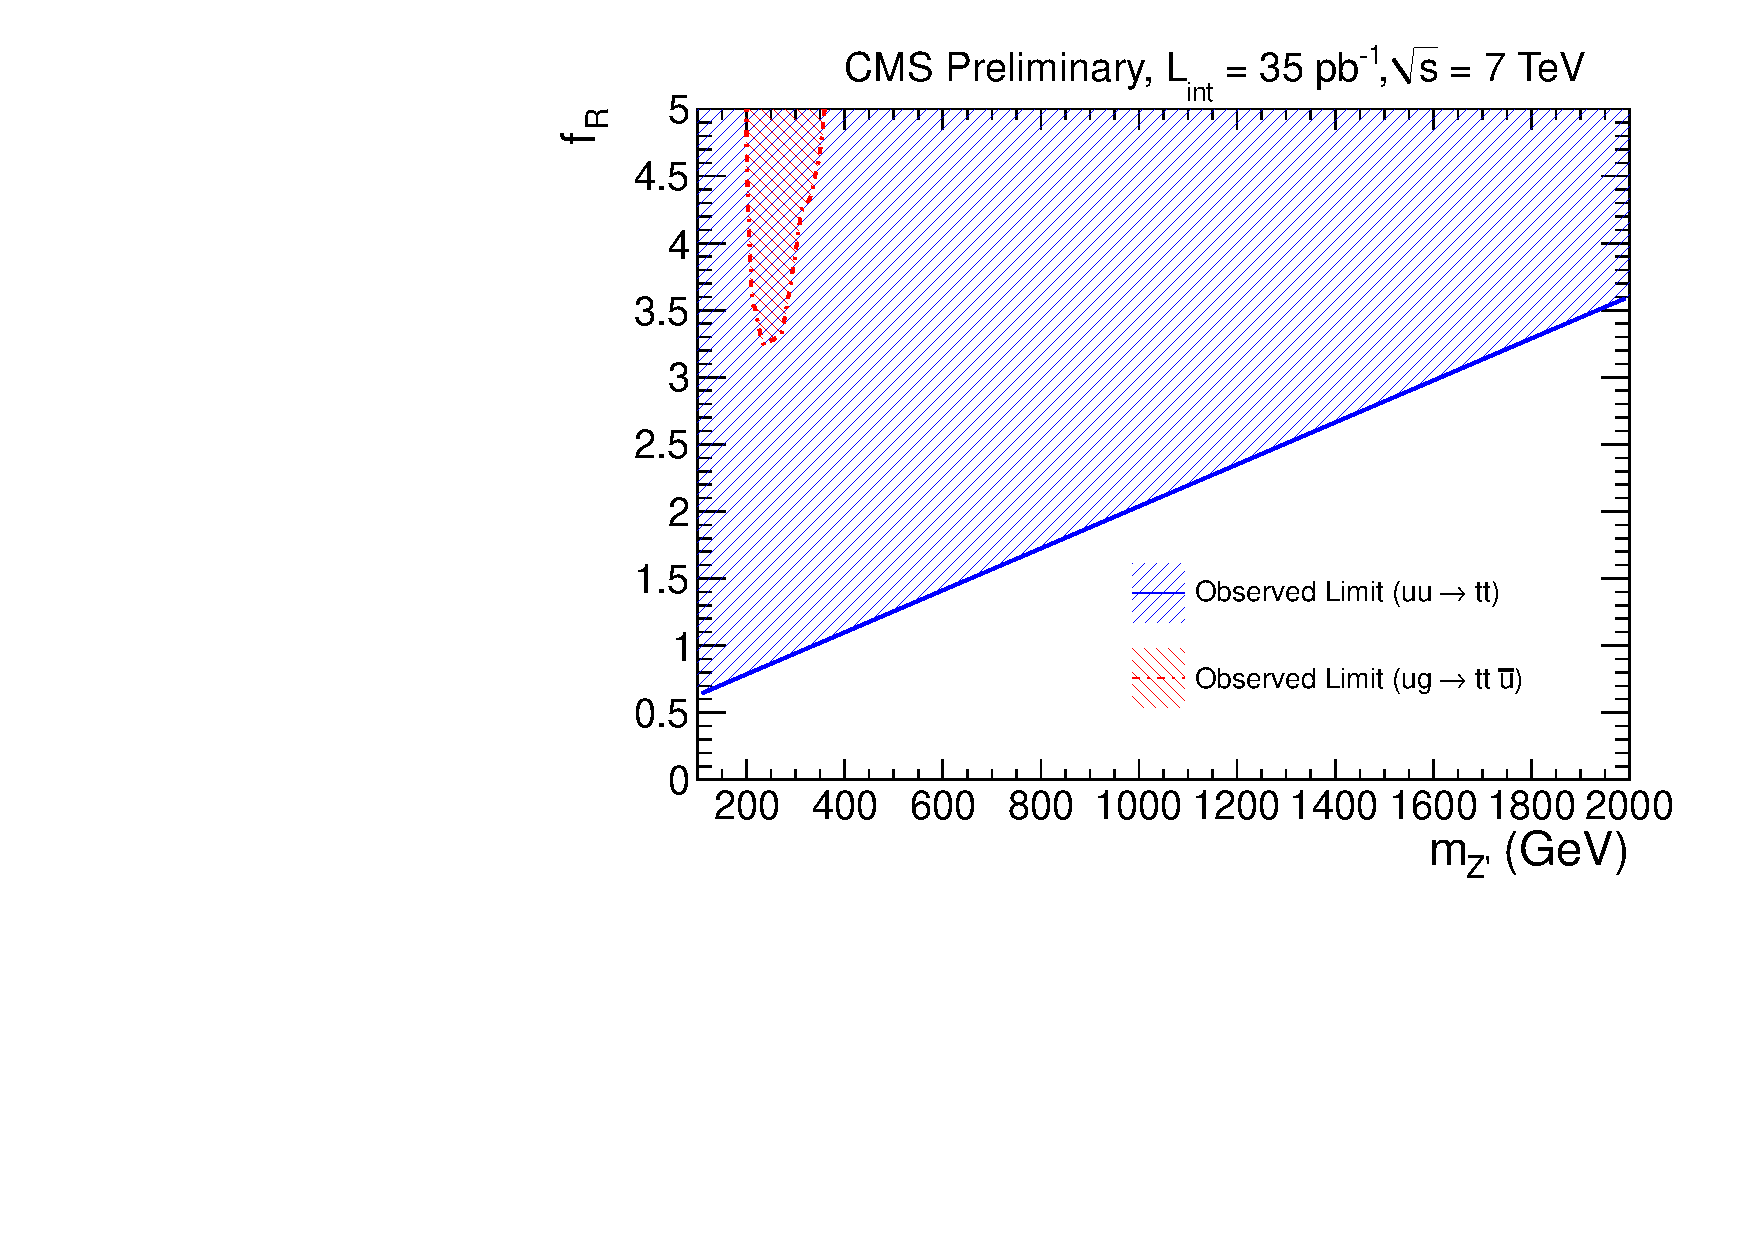
\includegraphics[width=0.7\linewidth]{figs/sstop_result.pdf}
\caption{ The exclusion region at 95\% CL. as a function of $Z'$ mass for various choices of the 
right-handed coupling, $f_R$. The solid lines represents regions due to t-channel exchange, where
as the dotted line excludes the assumptions on $ttj$ pair production. For the renormalization and factorization 
scales, $\mu$ is set to the top mass. \label{fig:sstopexclusion}}
\end{center}
\end{figure}

\begin{figure}[htb]
\begin{center}
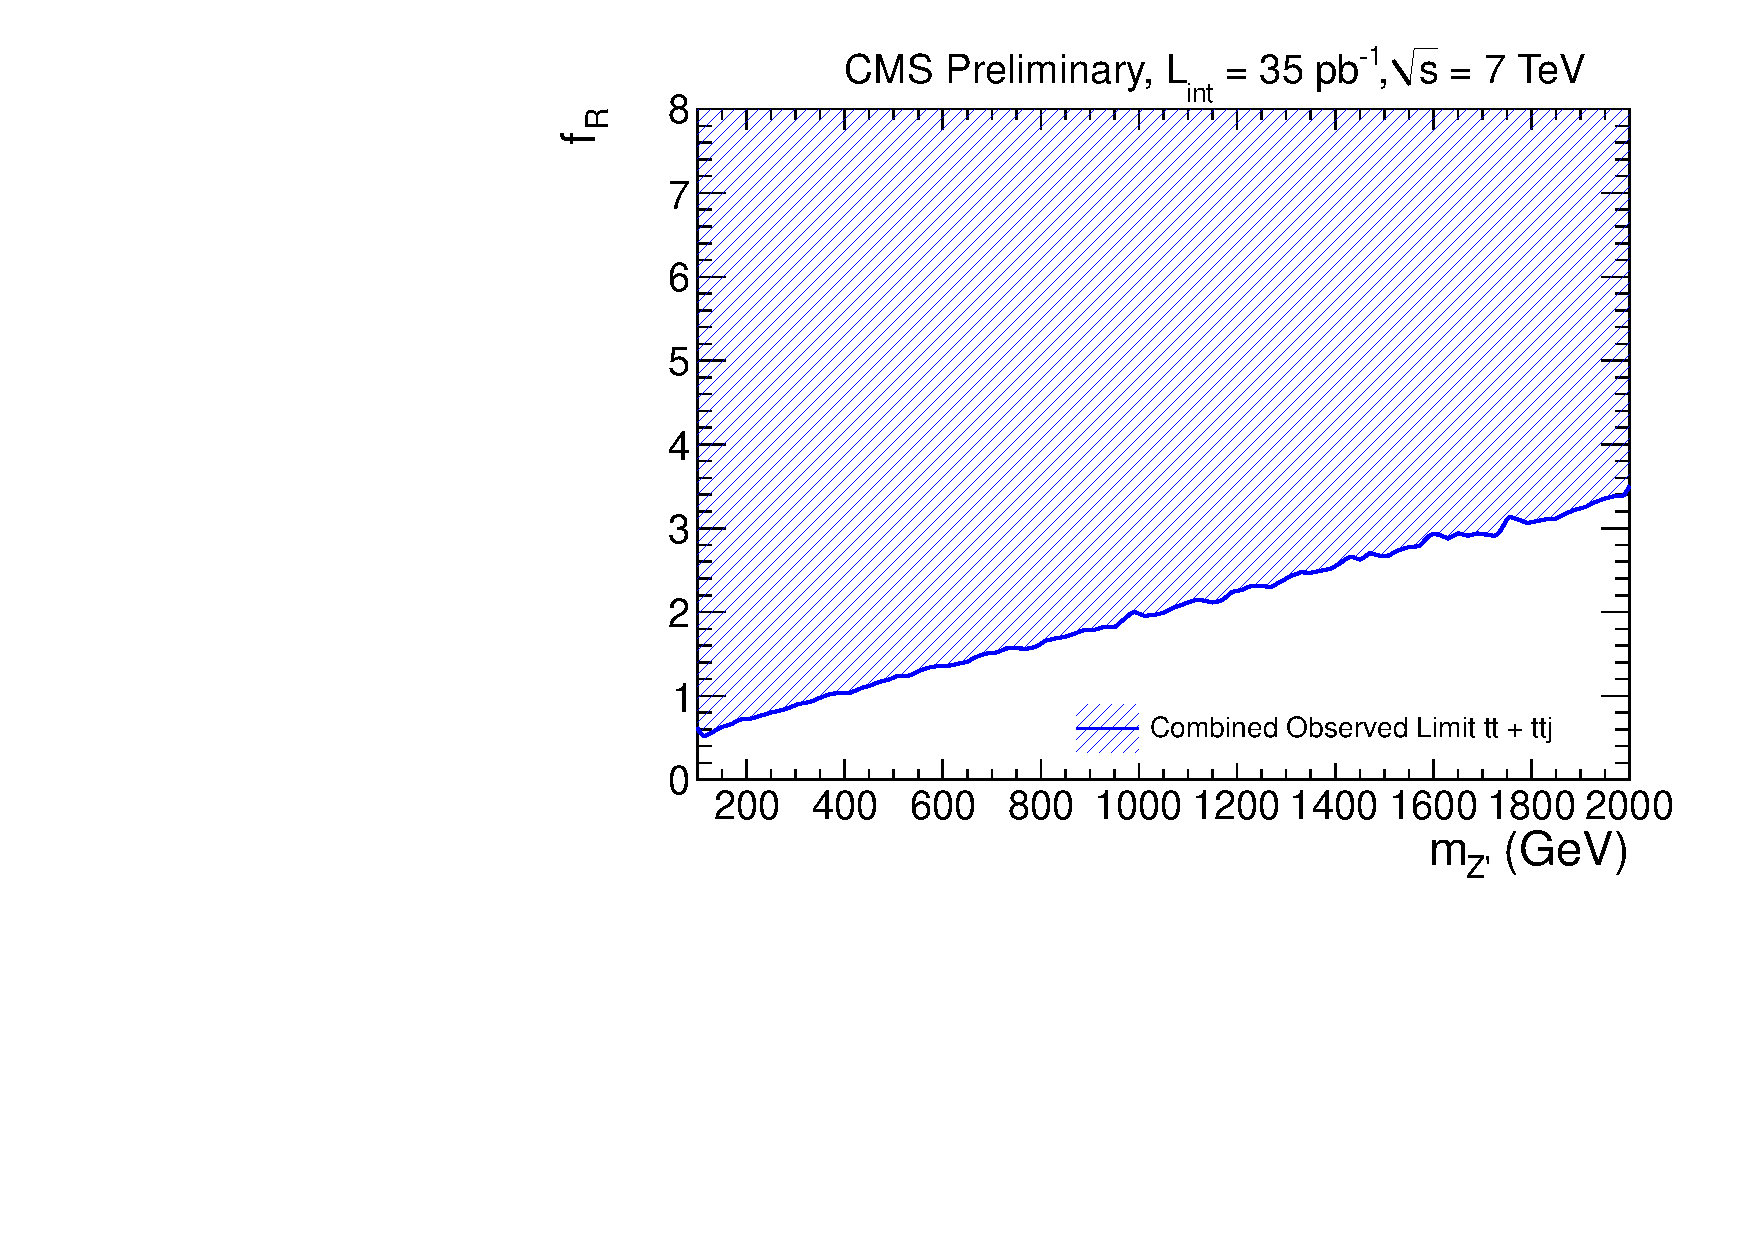
\includegraphics[width=0.7\linewidth]{figs/sscomb.pdf}
\caption{ The combined exclusion region at 95\% CL. as a function of $Z'$ mass for various choices of the 
right-handed coupling, $f_R$. Both t- and s-channel diagrams are added to get the combined exclusion limit
on same sign top production at the LHC. For the renormalization and factorization 
scales, $\mu$ is set to the top mass. \label{fig:sstopcombexclusion}}
\end{center}
\end{figure}

\section{Conclusion}
\label{sec:conclusion}

We have assessed the sensitivity to mSUGRA of a generic signal characterized by two isolated, high $p_T$ leptons,
significant jet activity, and \met. We performed a scan of the mSUGRA $m_{0}-m_{1/2}$ parameter space and determined  
the expected excluded region in the case of no observed signal as well as the $5\sigma$ sensitivity reach for both SS
and OS dileptons, assuming integrated luminosities of 100 pb$^{-1}$ and 1 fb$^{-1}$. Our results indicate that we are sensitive to a
significant region of the mSUGRA parameter space which extends upon previous results from the Tevatron. 



\clearpage
\begin{thebibliography}{99}

\bibitem{cdf:recentSusy} {CDF Trilepton Search, 2009, CDF/PUB/EXOTIC/PUBLIC/9817};\\
{\small \tt http://www-cdf.fnal.gov/physics/exotic/r2a/20090521.trilepton\_3fb/Welcome.html}
%\bibitem{cdf:recentSusy1} {``Inclusive Search for Squark and Gluino Production in $p\bar{p}$ Collisions at $\sqrt{s}$ = 1.96-TeV'', Phys.Rev.Lett.102:121801, (2009).}
\bibitem{d0:recentSusy} {``Search for associated production of charginos and neutralinos in the trilepton final state using 2.3 fb$^{-1}$ of data'', Phys. Lett. B 680, 34 (2009).}
%\bibitem{d0:recentSusy1} {``Search for squarks and gluinos in events with jets and missing transverse energy using 2.1 fb$^{-1}$ of ppbar collision data at $sqrt(s)=1.96$ TeV'', 
%Phys. Lett. B 660 , 449 (2008).}

\bibitem{osnote} {``Data driven background estimate for a new physics search with opposite sign dileptons''}, CMS AN-2009/130.

\bibitem{ssnote} {``Data driven background study for new physics searches with same sign dileptons at $\sqrt{s} = 10 $ TeV''}, CMS AN-2009/138.

\bibitem{mcsusy}{\tt https://twiki.cern.ch/twiki/bin/viewauth/CMS/SUSYMCRequirements0911}.

\bibitem{fast10}{\tt https://twiki.cern.ch/twiki/bin/view/CMS/SUSY33XScan}.

\bibitem{ww} {``Prospects for measuring the $WW$ production cross section in $pp$ collisions at $\sqrt s = $10 TeV''}, CMS AN-2009/042 and PAS EWK-09-002.

\bibitem{ttbar} {``Expectations for observation of top quark pair production in the dilepton final state with the early CMS data''}, CMS AN-2009/050 and PAS TOP-09-002.

\bibitem{tcmet} {``Correcting Missing Transverse Energy Using Tracks``} CMS AN-2009/022.

\bibitem{conversionnote} {``Study of photon conversion rejection at CMS''}, CMS AN-2009/159.

\bibitem{glbtrk} {\tt https://hypernews.cern.ch/HyperNews/CMS/get/muon/258.html}.

\bibitem{muonid} {``Muon Identification in CMS''}, CMS AN-2008/098.

\bibitem{vplusj} {\tt https://twiki.cern.ch/twiki/bin/view/CMS/VplusJets}.

\bibitem{fakenote} {``Data-driven methods to estimate the electron and muon fake contributions to lepton analyses''}, CMS AN-2009/041.

\bibitem{cite:cousins} {``Evaluation of three methods for calculating statistical significance when incorporating a systematic uncertainty into a test of the background-only hypothesis for a Poisson process''} arXiv:physics/0702156 [physics.data-an]

\bibitem{cite:conway} {``Interval estimation in the presence of nuisance parameters. 1. Bayesian approach''} arXiv:physics/0409129v1 [physics.data-an]

\bibitem{lep:lepsusyreach}{LEP Susy working group: {\tt http://lepsusy.web.cern.ch/lepsusy/} }

\bibitem{bayes}{\tt http://arxiv.org/pdf/physics/0409129}

\bibitem{victor} {\tt http://arxiv.org/pdf/0906.5016}; \\
{\tt http://indico.cern.ch/contributionDisplay.py?contribId=2\&confId=39042}.

\bibitem{summer09}{\tt https://twiki.cern.ch/twiki/bin/view/CMS/SUSY31XProduction}.


\end{thebibliography}

\end{document}
